\documentclass[11pt, a4paper, twocolumn]{article}
\raggedbottom

\usepackage[utf8]{inputenc}
\usepackage{amsfonts}
\usepackage{blindtext}
\usepackage{geometry}
\usepackage{setspace}
% \usepackage{titlesec}
\usepackage{indentfirst}
\usepackage{graphicx}
\usepackage[italian]{babel}
\usepackage{catchfile} % used in \getenv command
\usepackage{multicol}
\usepackage{amsmath}
\usepackage{subcaption}
\usepackage[hang, flushmargin, multiple, bottom]{footmisc}
\usepackage{float}
\usepackage{array}
\usepackage{booktabs}
\usepackage{url}
\usepackage{csvsimple}
\usepackage{framed}
\usepackage{xurl}

%\titlespacing*{\section}{0px}{3mm}{1mm}
%\titlespacing*{\subsection}{0px}{3mm}{1mm}
\geometry{
  left=2cm,
  right=2cm,
  top=2cm,
  bottom=2cm
}

\graphicspath{ {./assets}, {../../assets} }

% hyphen in bib
\makeatletter
\newcommand*\nobreakhyphen{\hbox{-}\nobreak\hskip\z@skip}
\makeatother

% Allow use of command \getenv{VARNAME}.
% Taken from: https://tex.stackexchange.com/questions/62010/can-i-access-system-environment-variables-from-latex-for-instance-home
\newcommand{\getenv}[2][]{
  \CatchFileEdef{\temp}{"|kpsewhich --var-value #2"}{\endlinechar=-1}%
  \if\relax\detokenize{#1}\relax\temp\else\let#1\temp\fi}

% Roman numerals
\newcommand{\rom}[1]{\uppercase\expandafter{\romannumeral #1\relax}}

% authors, date and title---------------------------------------------------------------
\author{Matteo Bonacini \\ \getenv{MAT1}}
\date{\today}
\title{Controllo di un pendolo invertito su rotaia}
%---------------------------------------------------------------------------------------
\begin{document}

  \twocolumn[
    \begin{@twocolumnfalse}

      \maketitle
      \begin{abstract}\label{sec:abstract}
  In questo progetto ho realizzato un pendolo fisico invertito su rotaia.
  Ho studiato il sistema in prossimità del punto di equilibrio instabile e ho usato la teoria del controllo per
  stabilizzarlo.
  Ho studiato due strategie di controllo: una \emph{ottimale} (\textsc{lqr}) e una \emph{non ottimale} (\textsc{pid}).
  Sono riuscito a stabilizzare il sistema con entrambe le strategie.
  Sebbene realizzare un controller \textsc{lqr} sia più difficile rispetto a un \textsc{pid}, i risultati che si
  ottengono sono migliori.
\end{abstract}


    \end{@twocolumnfalse}
  ]

  \section{Introduzione}\label{sec:introduzione}
\subsection{Pendolo invertito}\label{subsec:intro-pendolo}
Il pendolo invertito su rotaia è un sistema che si presta molto bene ad essere trattato nell'ambito della Teoria del
Controllo.
Il problema che ci poniamo è il seguente:
\begin{framed}
\emph{
    Un pendolo è posto su un carrello libero di muoversi orizzontalmente su una rotaia.
    Il carrello è dotato di un motore che gli permette di accelerare. Conoscendo lo stato del sistema
    $\mathbf x$, trovare un espressione per la forza che deve essere esercitata dal motore $u = u(\mathbf x)$
    che faccia sì che il pendolo si orienti verso l'alto.
  }
\end{framed}
Sebbene sia possibile risolvere questo problema per qualsiasi condizione iniziale del sistema, io tratterò solo il
caso in cui il pendolo parte già in prossimità della posizione verticale. Strategie di \emph{swing-up} e
\emph{swing-down} non saranno oggetto del mio studio.

\subsection{Controller \textsc{LQR}}\label{subsec:intro-lqr}
In generale, nello studio del controllo di un sistema, dobbiamo tenere a mente che la forzante
$\mathbf u$\footnote{La forzante è una matrice, in forma generale. Nel nostro caso, si riduce allo scalare $u$.}
che agisce su di esso, ha un certo costo associato.
Questo è da intendersi sia come costo \emph{materiale} (i.e. il costo della corrente per mettere in moto
un motore) ma, soprattutto, anche come costo \emph{fisico} (i.e. non si può realizzare un motore che ha potenza
infinita).

Un controller \textsc{lqr}, schematizzato in figura \ref{fig:lqr}, permette di risolvere questo problema in modo \emph{ottimale}.
Per spiegare cosa si intende con \emph{ottimale}, citerò direttamente la definizione di \textsc{lqr}:

\begin{framed}
  \textbf{DEF}
  Un controller \textsc{lqr} è una legge di controllo con input $\mathbf x$ e output $\mathbf u$\ldots
  \begin{equation}
    \begin{aligned}[c]
      \mathbf u = -K \mathbf x
    \end{aligned}
    \label{eq:lqr}
  \end{equation}
  \ldots dove la matrice $K$ è costruita in modo tale da minimizzare la seguente funzione costo:
  \begin{equation}
    J(t) \doteq
      \int_0^{+\infty} \left[ \mathbf{x} (s)^* Q \mathbf {x} (s) + \mathbf {u} (s)^* R \mathbf {u} (s) \right] ds
    \label{eq:lqr-costo}
  \end{equation}
  $Q$ ed $R$ sono matrici semidefinite positive che rappresentano, rispettivamente, il costo associato alla
  deviazione dello stato del sistema da $0$ e il costo dell'attuazione del controllo.
\end{framed}

\begin{figure}[h]
  \includegraphics[width=0.47\textwidth]{../assets/diagramma lqr.pdf}
  \caption{\emph{Controller \textsc{lqr}. Lo stato del sistema $\bf x$ è usato dal controller per decidere quale forzante
  $\bf u$ applicare, in modo da ottenere controllo ottimale.}}
  \label{fig:lqr}
\end{figure}

Per poter realizzare un controller di questo tipo, è necessario che il sistema in questione sia \emph{controllabile}.
Darò qualche nozione in più circa la controllabilità nella sezione \ref{subsec:controllabilità}, senza però entrare
troppo nel dettaglio.
Inoltre, ci tengo a precisare che sebbene le equazioni \eqref{eq:lqr} e \eqref{eq:lqr-costo}
valgano per sistemi dinamici a \emph{tempo continuo}, si possono generalizzare tranquillamente a sistemi
a \emph{tempo discreto}.
Rimando a Brunton\cite{brunton2019data} per approfondimenti.

\subsection{Controller \textsc{pid}}\label{subsec:intro-pid}
Un controller \textsc{pid} è un meccanismo di controllo in cui la forzante $\bf u$ è proporzionale a una funzione
errore $e(t)$, definita come differenza tra stato osservato $y(t)$ e stato desiderato $r(t)$ (figura \ref{fig:pid}).

\begin{framed}
  \textbf{DEF}
  Un controller \textsc{pid} è una legge di controllo definita come:
  \begin{equation}
    \begin{aligned}[c]
      u(t) = K_p e(t) + K_d \dot e(t) + K_i \int_0^t e(s)\ ds
    \end{aligned}
    \label{eq:pid}
  \end{equation}
  $K_p$, $K_d$ e $K_i$ sono coefficienti reali positivi.
\end{framed}


\begin{figure}[h]
  \includegraphics[width=0.47\textwidth]{../assets/diagramma pid.pdf}
  \caption{\emph{Controller \textsc{pid}. $r(t)$ è lo stato desiderato, $y(t)$ è lo stato misurato.}}
  \label{fig:pid}
\end{figure}

Un controller di questo tipo non gode dello stesso background matematico di un controller del tipo \eqref{eq:lqr}.
Il suo vantaggio sta nel fatto che per realizzarlo non è necessaria alcuna conoscenza a priori del modello del sistema.

  \section{Modello e implementazione del sistema}\label{sec:modello}
\subsection{Modello del sistema}\label{subsec:modello-del-sistema}
Il sistema del pendolo invertito è riassunto in figura \ref{fig:sistema}.
In questa sezione, ricaverò le equazioni del moto e le linearizzerò attorno al punto di equilibrio instabile.

\begin{figure}[h]
    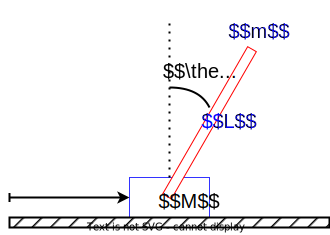
\includegraphics{../assets/sistema.pdf}
  \caption{\emph{Pendolo invertito. Le variabili generalizzate sono $x$ e $\theta$. Il carrello ha massa $M$,
  il pendolo ha lunghezza $L$ e massa $m$. Un motore (non rappresentato in figura) esercita una forza che agisce
  lungo $\hat x$. Si noti che la variabile generalizzata $x$ e lo stato del sistema $\bf x$ sono due grandezze diverse.}}
  \label{fig:sistema}
\end{figure}


La Lagrangiana del sistema è\footnote{Per semplificare i calcoli, avrei potuto scrivere direttamente la Lagrangiana delle
piccole oscillazioni attorno al punto di equilibrio instabile, ottenendo lo stesso risultato. Facendo così, però, non avrei
ottenuto le equazioni non lineari del moto, che mi sono servite per simulare il sistema a computer.}
\begin{equation}
  \begin{aligned}
    \mathcal L &= T - V\\
      &= \frac 1 2 \left[
        M \dot x^2 + mv_{p}^2 + I_{p} \dot \theta^2
      \right] -\\
      &- mg\frac L 2\cos{\theta}
    \end{aligned}
  \label{eq:lagrangiana}
\end{equation}
dove $v_p$ e $I_p$ indicano rispettivamente velocità del centro di massa e momento d'inerzia calcolato rispetto al
centro di massa del pendolo.
In particolare, valgono:
\begin{equation}
  \begin{aligned}
    v_p^2 &= \left(\dot x + \frac L 2 \dot \theta \cos{\theta}\right)^2 + \left(\frac L 2 \dot \theta \sin{\theta}\right)^2 \\
    I_p &= \frac 1 {12} m L^2
  \end{aligned}
  \label{eq:lagrangiana-2}
\end{equation}

Imposto e risolvo le equazioni di Eulero:
\begin{equation}
  \left\{
    \begin{aligned}
      \frac d {dt} \frac {\partial \mathcal L} {\partial \dot x } - \frac {\partial \mathcal L} {\partial  x}&= f \\
      \frac d {dt} \frac {\partial \mathcal L} {\partial \dot \theta } - \frac {\partial \mathcal L} {\partial \theta}&= 0
    \end{aligned}
  \right.
  \label{eq:eulero}
\end{equation}

In questo modo trovo le equazioni del moto non lineari:
\begin{equation}
  \left\{
  \begin{aligned}
    \ddot x &= \frac{2m\sin\theta\left(3g\cos\theta-2l\dot \theta^2\right)-8f}{3m\cos(2\theta)-5m-8M} \\
    \ddot \theta &= \frac{3\sin\theta \left(lm\dot \theta^2\cos\theta-2g(m+M)\right)+6f\cos\theta}{l\left(3m\cos^2\theta-4(m+M)\right)}
  \end{aligned}
  \right.
  \label{eq:moto}
\end{equation}

Ora faccio un cambio di variabile, in modo da avere un sistema di primo ordine.
Ho usato il simbolo $(\ldots)$ al posto di riscrivere le equazioni \eqref{eq:moto} nel sistema.
\begin{equation}
  \dot {\mathbf x} = \left(
  \begin{matrix}
    \dot x \\
    \dot v \\
    \dot \theta \\
    \dot \omega
  \end{matrix}\right) = \left(
  \begin{matrix}
    v \\
    (\ldots) \\
    \omega \\
    (\ldots)
  \end{matrix}
  \right)
  \label{eq:state-space}
\end{equation}

I punti di equilibrio del sistema \eqref{eq:state-space} si trovano imponendo: $\dot x = 0 \land \dot \theta = 0
\land f = 0$ e sono:
\begin{equation}
  \begin{aligned}
    \mathbf x_I &= (x, 0, 0, 0) \to & \text{instabile} \\
    \mathbf x_S &= (x, 0, \pi, 0) \to & \text{stabile}
  \end{aligned}
  \label{eq:punti-equilibrio}
\end{equation}

Linearizzo le equazioni \eqref{eq:state-space} attorno a $\mathbf x_I$.
Calcolo la Jacobiana:
\begin{equation}
  J_{\dot{\mathbf x}}(\mathbf x_I) =
  \left(\begin{array}{ccccc}0&1&0&0&0\\0&0&-\frac{3gm}{m+4M}&0&\frac{4}{m+4M}\\0&0&0&1&0\\0&0&-\frac{6g(m+M)}{l(m+4M)}&0&\frac{6}{lm+4lM}\\\end{array}\right)
  \label{eq:jacobiana}
\end{equation}

In prossimità di $\mathbf x_I$, posso quindi approssimare le equazioni del moto del sistema nella forma
$\dot {\mathbf x} = A\mathbf x + B f$. $A$ e $B$ valgono:
\begin{equation}
  A =
  \left(\begin{array}{cccc}0&1&0&0\\0&0&-\frac{3gm}{m+4M}&0\\0&0&0&1\\0&0&-\frac{6g(m+M)}{l(m+4M)}&0\\\end{array}\right)
  \hspace{10px}
  B =
  \left(\begin{array}{c}0\\\frac{4}{m+4M}\\0\\\frac{6}{lm+4lM}\\\end{array}\right)
  \label{eq:A-e-B}
\end{equation}

\subsection{Implementazione del sistema}\label{subsec:implementazione-del-sistema}
Ho realizzato il sistema modellato in sezione \ref{subsec:modello-del-sistema}, così come descritto in fig. %todo add figura
La scelta dei componenti garantisce che l'attrito sia trascurabile.
Una serie di sensori permette di misurare lo stato del sistema.
Per maggiori dettagli sui componenti utilizzati, consultare l'appendice %todo add ref.



  \section{Sviluppo del controller \textsc{LQG}}\label{sec:lqg}
\subsection{Discretizzazione del sistema}\label{subsec:discretizzazione}
Nella sezione \ref{subsec:intro-lqr} ho spiegato come funziona un controller \textsc{lqr} per sistemi a \emph{tempo continuo}.
Il sistema che ho realizzato, tuttavia, non può raccogliere dati dai sensori in modo continuo: tra un osservazione
$\mathbf x_k$ e la successiva $\mathbf x_{k+1}$ passa un certo intervallo di tempo $\Delta t$.
Tutte le considerazioni fatte finora continuano a valere, ma dal punto di vista pratico è necessario discretizzare il sistema.
Vogliamo trovare le matrici $A_d$ e $B_d$ tali cui le equazioni
\begin{equation}
  \begin{aligned}
    \mathbf{x}_{k+1} = A_d \mathbf{x}_k + B_d u_k
  \end{aligned}
  \label{eq:moto-discreto}
\end{equation}
approssimino meglio le \eqref{eq:state-space} fissato un $\Delta t > 0$.
Si può dimostrare\cite{brunton2019data}
che valgono:
\begin{equation}
  \begin{aligned}
    A_d &= e^{A\Delta t} \\
    B_d &= B\left( \int_0^{\Delta t} e^{A s} ds \right)
  \end{aligned}
  \label{eq:discrete-mapping}
\end{equation}
Tuttavia, operativamente, per $\Delta t \ll 1$, possiamo trovare velocemente una soluzione approssimata per \eqref{eq:discrete-mapping}:
\begin{equation}
  \begin{aligned}
    \mathbf x_{k+1} &\approx \mathbf x_k + \dot {\mathbf x}|_k \Delta t\\
      &\approx \mathbf x_k + (A \mathbf x_k + B u_k) \Delta t\\
      &\approx (I + \Delta t A) \mathbf x_k + B \Delta t u_k\\
  \end{aligned}
  \label{eq:discrete-mapping-approx}
\end{equation}
Le matrici che cerchiamo sono quindi:
\begin{equation}
  \begin{aligned}
  A_d &=
  \left(\begin{array}{cccc}1&\Delta t&0&0\\0&1&-\frac{3gm}{m+4M}\Delta t&0\\0&0&1&\Delta t\\0&0&-\frac{6g(m+M)}{l(m+4M)} \Delta t&1\\\end{array}\right)
  \\
  B_d &=
  \left(\begin{array}{c}0\\\frac{4}{m+4M} \Delta t\\0\\\frac{6}{lm+4lM} \Delta t\\\end{array}\right)
  \label{eq:Ad-e-Bd}
  \end{aligned}
\end{equation}

\subsection{Controllabilità del sistema}\label{subsec:controllabilità}
Prima di procedere con il calcolo dei coefficienti del controller, dobbiamo accertarci che il sistema sia \emph{controllabile}.
Condizione necessaria e sufficiente per la controllabilità è che la \emph{matrice di controllabilità}, definita in \eqref{eq:matrice-controllabilità}
abbia rango massimo\footnote{
  In realtà, è necessario anche che gli autovalori di $A$ non abbiano la forma $\frac {2k\pi i} {\Delta t}, \forall k \in \mathbb Z_0$.
  Si può verificare facilmente questa condizione fissando qualche valore numerico; per
  ora assumerò che sia soddisfatta (in ogni caso, gli autovalori di $A$ dipendono solo da parametri razionali, quindi è
  pressochè impossibile che assumano valori multipli di $\pi$).
}%
\footnote{
  Questo test per la controllabilità non mi da alcuna informazione su \emph{quanto} sia controllabile il mio sistema.
  Esistono altri metodi che permettono di ottenere queste informazioni (e.g. si può calcolare il Gramiano
  $W=\int_0^{+\infty}e^{As}BB^*e^{A^*s}\ ds$ e studiarne gli autovalori).
}
\cite{sontag2013mathematical}.

\begin{framed}
  \textbf{DEF} Matrice di controllabilità
  \begin{equation}
    \mathcal C_d \doteq \left[
      \begin{matrix}
        B_d & A_dB_d & A_d^2B_d & \ldots & A_d^{n-1}B_d
      \end{matrix}
      \right]
    \label{eq:matrice-controllabilità}
  \end{equation}
\end{framed}

Svolgendo i calcoli, si trova che il sistema \eqref{eq:A-e-B} è sempre controllabile\footnote{Assumendo che tutti i
parametri siano positivi.}.

\subsection{Calcolo dei coefficienti del controller}\label{calcolo-coefficienti}
Definisco la funzione costo per il sistema \eqref{eq:discrete-mapping}:
\begin{equation}
  J(t) =
  \sum_{k=0}^{+\infty} \left[ \mathbf{x}_k^* Q \mathbf {x}_k + u_k R u_k \right]
  \label{eq:lqr-costo-discreto}
\end{equation}
si può dimostrare\cite{chow1975analysis} che la soluzione $u = u(\mathbf x)$ ottimale per il problema di controllo al tempo $t = k \Delta t$ è data da:
% yeet subscript t per infinite horizon problem
\begin{equation}
  \begin{aligned}
  u_k^{\text{opt}}(\mathbf x) &= -K y_{k-1} \\
  \text{con}\ K &= (B_d^*PB_d + R)^{-1}(B_d^*PA_d)
  \end{aligned}
  \label{eq:f-opt}
\end{equation}
dove $P$ è la soluzione all'equazione di Ricciati a tempo discreto (\textsc{dare})\eqref{eq:ricciati}:%
\begin{framed}
  \textbf{DEF} \textsc{dare}
  \begin{equation}
    \begin{aligned}
    P &=A_d^* P A_d\ - \\
     &-(A_d^* P B_d)(R + B_d^* P B_d)^{-1}(B_d^* P A_d)\ + \\
    &+ Q
    \end{aligned}
    \label{eq:ricciati}
  \end{equation}%
\end{framed}%
Calcolare i coefficienti del controller significa risolvere l'equazione \eqref{eq:ricciati} e trovare il vettore $K$
\footnote{In realtà, manca un ultimo dettaglio implementativo: bisogna trovare una relazione tra la forzante $u$ e
la tensione $V$ da applicare al motore. I dettagli sono abbastanza noiosi e li ho riassunti in appendice \ref{sec:calibrazione-motore}.}.


  \section{Sviluppo del controller \textsc{PID}}\label{sec:pid}
4

  \section{Risultati}\label{sec:risultati}
5

  \section{Conclusioni}\label{sec:conclusioni}
5

  \appendix
last

\subsection{First Appendix}
\label{FirstAppendix}

\subsubsection{First Subsection In Appendix}
\label{FirstSubsectionAppendix}




\bibliographystyle{unsrt} % We choose the "plain" reference style
\bibliography{invertedPendulumRefs}
\end{document}
